\section{Results} \label{sec:results}
There is no standard benchmark to evaluate merging approaches on models from distinct tasks, so we construct our own. We evaluate our approach in two different settings.
% Thus, we test our method in two different settings:
(1) A versatile test-bed: disjoint category splits of the same dataset (i.e., \textit{same dataset and different label sets}).
(2) A very challenging setting: completely different datasets and tasks (i.e., \textit{different datasets and label sets}). 

% (1) A versatile test-bed setting: disjoint category splits of the same dataset (i.e., \textit{same dataset and different label sets}).
% (2) A very challenging setting: completely different datasets (i.e., \textit{different datasets and label sets}). 


% There is no standard setting to evaluate merging approaches on models from distinct tasks. 
% % Thus, we devise two types of experiments to benchmark merging approaches:
% Thus, we devise two types of benchmarks:
% % Thus, we devise two types of experiments to benchmark disjoint task model merging (Fig.~\ref{fig:concept_and_capabilities}):
% (1) Merging models trained on disjoint category splits of the same dataset (i.e., \textit{same dataset and different label sets}), and (2) merging models trained on completely different datasets (i.e., \textit{different datasets and label sets}). 
% We position the former as an easy-to-use versatile test-bed for evaluating merging methods, and the latter as a very challenging setting.

% We position the former as versatile and standardized test-bed for judging the quality of arbitrary merging methods for arbitrary architectures, and the latter to showcase \name{}'s performance in realistic settings.

\paragraph{Experimental Details.} 
For each experiment where we sample multiple disjoint splits of categories, we hold one split out for hyperparameter search and report mean and standard deviation on the rest. 
For experiments with models trained on different datasets, we subsample the validation set into a validation and test set to use for the same purpose.
To compute correlations, we use a portion of the training set for each dataset as in \citet{li2016convergenticlr} (see Appendix~\ref{ap:data_usage}).
For a fair comparison, we reset the batch norms for \textit{all} methods (including the original models) using the training data (following the recommendation in \citet{jordan2022repair}).
For our method, \name{}$_\text{n/m}$ indicates that $n$ out of the $m$ layers in the network have been zipped (Sec.~\ref{sec:partial_zip}).
Note, all our models have \textit{different initializations}.

\paragraph{Evaluation.}
For the setting with disjoint class splits of the same dataset, we evaluate performance in two ways: joint accuracy and per task accuracy. For joint accuracy, we evaluate each model over \textit{all} classes in the combined dataset. For per task accuracy, we compute the accuracy of each task individually (i.e., supposing we had task labels at runtime) and then report the average. The former is similar to a continual learning setting where we want to augment the knowledge of the model, while the latter is akin to a multi-task setting where we know which task we're using at test time.
For the scenario where we merge models trained on different datasets, we use the per task accuracy metric, as the label spaces are not comparable.

\paragraph{Baselines.} In addition to the default Weight Matching version of Git Re-Basin \cite{ainsworth2022git}, we compare to two baselines: Weight Averaging (Eq.~\ref{eq:wavg}) and Permute (Eq.~\ref{eq:rebasin}) with $\gamma = \sfrac{1}{2}$ using our framework (i.e., we set \modelc{$M_i$} and \modelc{$U_i$} such that Eq.~\ref{eq:zip} is equivalent). For Permute, we use linear sum assignment to find optimal permutations (following \citet{li2016convergenticlr}). Note that our Permute is a \textit{strong} baseline we create using our framework and is more accurate than Git Re-Basin in our settings. It's also similar to REPAIR \cite{jordan2022repair}, but without adding extra parameters to the model. Finally, with perfect merging, the merged model's outputs would be identical to the originals. Thus we include Ensemble as an \gc{upper bound} (executing and concatenating the results of both models).

%##################################################################################################
\begin{table*}[t]
\centering
\subfloat[
    \textbf{CIFAR-10 (5+5).} ResNet-20 (4$\times$ width).
    \label{tab:cifar5+5}
]{
\centering
\begin{minipage}{0.47\linewidth}{
\begin{center}
\resizebox{\textwidth}{!}{
    \tablestyle{5pt}{1.1}
    \begin{tabular}{lc|cccc}
        & & \multicolumn{4}{c}{Accuracies (\%)}\\
        Method & FLOPs (G) & Joint & \modela{Task A} & \modelb{Task B} & Avg \\
        \shline
        \modela{Model A} & {0.68} & {48.2\conf{1.0}} & {97.0\conf{0.6}} & {45.1\conf{8.6}} & {71.0\conf{4.4}} \\
        \modelb{Model B} & {0.68} & {48.4\conf{3.8}} & {49.1\conf{9.3}} & {96.1\conf{1.1}} & {72.6\conf{4.9}} \\
        \hline
        W. Avg \tiny{(Eq.~\ref{eq:wavg})} & 0.68 & {43.0\conf{1.6}} & {54.1\conf{1.4}} & {67.5\conf{1.2}} & {60.8\conf{4.5}} \\
        % Git Re-Basin \cite{ainsworth2022git}  & 0.68 & {46.2\conf{0.8}} & {76.8\conf{8.9}} & {82.7\conf{5.1}} & {79.8\conf{6.5}} \\
        Git Re-Basin$^{\ddag}$  & 0.68 & {46.2\conf{0.8}} & {76.8\conf{8.9}} & {82.7\conf{5.1}} & {79.8\conf{6.5}} \\
        Permute \tiny{(Eq.~\ref{eq:rebasin})} & 0.68 & {58.4\conf{6.8}} & {86.6\conf{2.1}} & {87.4\conf{1.1}} & {87.4\conf{1.4}} \\
        \default{{\bf \name{}}$_\text{20/20}$} & 0.68 & \textbf{79.1\conf{1.1}} & \textbf{92.9\conf{1.1}} & \textbf{91.2\conf{1.4}} & \textbf{92.1\conf{1.0}} \\
        \hline
        \gc{Ensemble} & \gc{1.37} & \gc{87.4\conf{2.6}} & \gc{97.0\conf{0.6}} & \gc{96.1\conf{1.1}} & \gc{96.6\conf{0.4}} \\
        \default{{\bf \name{}}$_\text{13/20}$} & 0.91 & \textbf{83.8\conf{3.1}} & \textbf{95.1\conf{0.7}} & \textbf{94.1\conf{1.5}} & \textbf{94.6\conf{0.6}} \\
    \end{tabular}
}
\end{center}
}\end{minipage}
}
\hspace{1em}
\centering
\subfloat[
    \textbf{CIFAR-100 (50+50).} ResNet-20 (8$\times$ width).
    \label{tab:cifar50+50}
]{
\centering
\begin{minipage}{0.47\linewidth}{
\begin{center}
\resizebox{\textwidth}{!}{
    \tablestyle{5pt}{1.1}
    \begin{tabular}{y{53}x{40}|x{30}x{30}x{30}x{30}}
        & & \multicolumn{4}{c}{Accuracies (\%)}\\
        Method & FLOPs (G) & Joint & \modela{Task A} & \modelb{Task B} & Avg \\
        \shline
        \modela{Model A} & {2.72} & {41.6\conf{0.3}} & {82.9\conf{0.7}} & {24.8\conf{0.4}} & {53.9\conf{0.5}} \\
        \modelb{Model B} & {2.72} & {41.6\conf{0.2}} & {25.1\conf{1.2}} & {82.8\conf{0.2}} & {54.0\conf{0.6}} \\
        \hline
        W. Avg \tiny{(Eq.~\ref{eq:wavg})}             &  2.72     & {17.0\conf{1.7}}          & {23.8\conf{6.9}}     & {24.8\conf{5.9}} & {24.3\conf{1.9}} \\
        % Git Re-Basin \cite{ainsworth2022git}        &  2.72     & {40.9\conf{0.2}}          & {57.3\conf{1.5}}      & {56.7\conf{0.7}}  & {57.0\conf{0.8}}  \\
        Git Re-Basin$^{\ddag}$    &  2.72     & {40.9\conf{0.2}}          & {57.3\conf{1.5}}      & {56.7\conf{0.7}}  & {57.0\conf{0.8}}  \\
        Permute \tiny{(Eq.~\ref{eq:rebasin})}    &  2.72     & {42.8\conf{0.7}}          & {61.6\conf{1.4}}      & {60.5\conf{0.5}}   & {61.0\conf{0.8}} \\
        \default{{\bf \name{}}$_\text{20/20}$}  &  2.72   & \textbf{54.9\conf{0.8}}          & \textbf{68.2\conf{0.8}}      & \textbf{67.9\conf{0.6}}  & \textbf{68.0\conf{0.4}} \\
        \hline
        \gc{Ensemble}                           & \gc{5.45} & \gc{73.5\conf{0.4}}       & \gc{82.9\conf{0.7}}   & \gc{82.8\conf{0.2}}& \gc{82.8\conf{0.4}} \\
        \default{{\bf \name{}}$_\text{13/20}$}  & {3.63}    & \textbf{70.2\conf{0.4}}   & \textbf{80.3\conf{0.8}}      & \textbf{80.1\conf{0.7}}  & \textbf{80.2\conf{0.6}} \\
    \end{tabular}
}
\end{center}
}\end{minipage}
}
\caption{\textbf{CIFAR Results.} \name{}\ vs.\ baselines
on combining a model trained on half the classes (\modela{Task A}) with one trained on the other half (\modelb{Task B}) \textit{without extra training}. We report both joint (10/100-way) and per-task (5/50-way) accuracy.
\name{}\ \textit{significantly} outperforms its baseline and closes in on the \gc{upper bound} (ensemble accuracy).
$\ddag$ refers to \citet{ainsworth2022git}.
}
\label{tab:cifar_results}
\vspace{-15pt}
\end{table*}
%##################################################################################################


% %##################################################################################################
% \begin{table*}[t]
% \centering
% \subfloat[
%     \textbf{CIFAR-10 (5+5).} Using ResNet-20 (4$\times$ width).
%     \label{tab:cifar5+5}
% ]{
% \centering
% \begin{minipage}{0.46\linewidth}{
% \begin{center}
% \resizebox{\textwidth}{!}{
%     \tablestyle{5pt}{1.1}
%     \begin{tabular}{y{56}x{20}x{28}|x{24}x{24}x{24}}
%         & FLOPs& Joint & \multicolumn{3}{c}{Per-Task (\%)}\\
%         Method & (G) & Acc (\%) & \modela{Task A} & \modelb{Task B} & Avg\\
%         \shline
%         \modela{Model A} & {0.68} & {48.2\conf{1.0}} & {97.0\conf{0.6}} & {45.1\conf{8.6}} & {71.0\conf{4.4}} \\
%         \modelb{Model B} & {0.68} & {48.4\conf{3.8}} & {49.1\conf{9.3}} & {96.1\conf{1.1}} & {72.6\conf{4.9}} \\
%         \hline
%         W. Avg \tiny{(Eq.~\ref{eq:wavg})} & 0.68 & {43.0\conf{1.6}} & {54.1\conf{1.4}} & {67.5\conf{1.2}} & {60.8\conf{4.5}} \\
%         % Git Re-Basin \cite{ainsworth2022git}  & 0.68 & {46.2\conf{0.8}} & {76.8\conf{8.9}} & {82.7\conf{5.1}} & {79.8\conf{6.5}} \\
%         Git Re-Basin$^{\ddag}$  & 0.68 & {46.2\conf{0.8}} & {76.8\conf{8.9}} & {82.7\conf{5.1}} & {79.8\conf{6.5}} \\
%         Permute \tiny{(Eq.~\ref{eq:rebasin})} & 0.68 & {58.4\conf{6.8}} & {86.6\conf{2.1}} & {87.4\conf{1.1}} & {87.4\conf{1.4}} \\
%         \default{{\bf \name{}}$_\text{20/20}$} & 0.68 & \textbf{79.1\conf{1.1}} & \textbf{92.9\conf{1.1}} & \textbf{91.2\conf{1.4}} & \textbf{92.1\conf{1.0}} \\
%         \hline
%         \gc{Ensemble} & \gc{1.37} & \gc{87.4\conf{2.6}} & \gc{97.0\conf{0.6}} & \gc{96.1\conf{1.1}} & \gc{96.6\conf{0.4}} \\
%         \default{{\bf \name{}}$_\text{13/20}$} & 0.91 & \textbf{83.8\conf{3.1}} & \textbf{95.1\conf{0.7}} & \textbf{94.1\conf{1.5}} & \textbf{94.6\conf{0.6}} \\
%     \end{tabular}
% }
% \end{center}
% }\end{minipage}
% }
% \hspace{1em}
% \centering
% \subfloat[
%     \textbf{CIFAR-100 (50+50).} Using ResNet-20 (8$\times$ width).
%     \label{tab:cifar50+50}
% ]{
% \centering
% \begin{minipage}{0.46\linewidth}{
% \begin{center}
% \resizebox{\textwidth}{!}{
%     \tablestyle{5pt}{1.1}
%     \begin{tabular}{y{56}x{20}x{28}|x{24}x{24}x{24}}
%         & FLOPs& Joint & \multicolumn{3}{c}{Per-Task (\%)}\\
%         Method & (G) & Acc (\%) & \modela{Task A} & \modelb{Task B} & Avg\\
%         \shline
%         \modela{Model A} & {2.72} & {41.6\conf{0.3}} & {82.9\conf{0.7}} & {24.8\conf{0.4}} & {53.9\conf{0.5}} \\
%         \modelb{Model B} & {2.72} & {41.6\conf{0.2}} & {25.1\conf{1.2}} & {82.8\conf{0.2}} & {54.0\conf{0.6}} \\
%         \hline
%         W. Avg \tiny{(Eq.~\ref{eq:wavg})}             &  2.72     & {17.0\conf{1.7}}          & {23.8\conf{6.9}}     & {24.8\conf{5.9}} & {24.3\conf{1.9}} \\
%         % Git Re-Basin \cite{ainsworth2022git}        &  2.72     & {40.9\conf{0.2}}          & {57.3\conf{1.5}}      & {56.7\conf{0.7}}  & {57.0\conf{0.8}}  \\
%         Git Re-Basin$^{\ddag}$    &  2.72     & {40.9\conf{0.2}}          & {57.3\conf{1.5}}      & {56.7\conf{0.7}}  & {57.0\conf{0.8}}  \\
%         Permute \tiny{(Eq.~\ref{eq:rebasin})}    &  2.72     & {42.8\conf{0.7}}          & {61.6\conf{1.4}}      & {60.5\conf{0.5}}   & {61.0\conf{0.8}} \\
%         \default{{\bf \name{}}$_\text{20/20}$}  &  2.72   & \textbf{54.9\conf{0.8}}          & \textbf{68.2\conf{0.8}}      & \textbf{67.9\conf{0.6}}  & \textbf{68.0\conf{0.4}} \\
%         \hline
%         \gc{Ensemble}                           & \gc{5.45} & \gc{73.5\conf{0.4}}       & \gc{82.9\conf{0.7}}   & \gc{82.8\conf{0.2}}& \gc{82.8\conf{0.4}} \\
%         \default{{\bf \name{}}$_\text{13/20}$}  & {3.63}    & \textbf{70.2\conf{0.4}}   & \textbf{80.3\conf{0.8}}      & \textbf{80.1\conf{0.7}}  & \textbf{80.2\conf{0.6}} \\
%     \end{tabular}
% }
% \end{center}
% }\end{minipage}
% }
% \caption{\textbf{CIFAR Results.} \name{}\ vs. baselines
% on combining a model trained on half the classes (\modela{Task A}) with one trained on the other half (\modelb{Task B}) \textit{without extra training}. We report both joint (10/100-way) and per-task (5/50-way) accuracy.
% \name{}\ \textit{significantly} outperforms its baseline and closes in on the \gc{upper bound} (ensemble accuracy).
% $\ddag$ refers to \cite{ainsworth2022git}
% }
% \label{tab:cifar_results}
% \vspace{-15pt}
% \end{table*}
% %##################################################################################################



% \begin{figure}[b]
% \centering

% \begin{minipage}{0.48\linewidth}{
%     % \centering
%     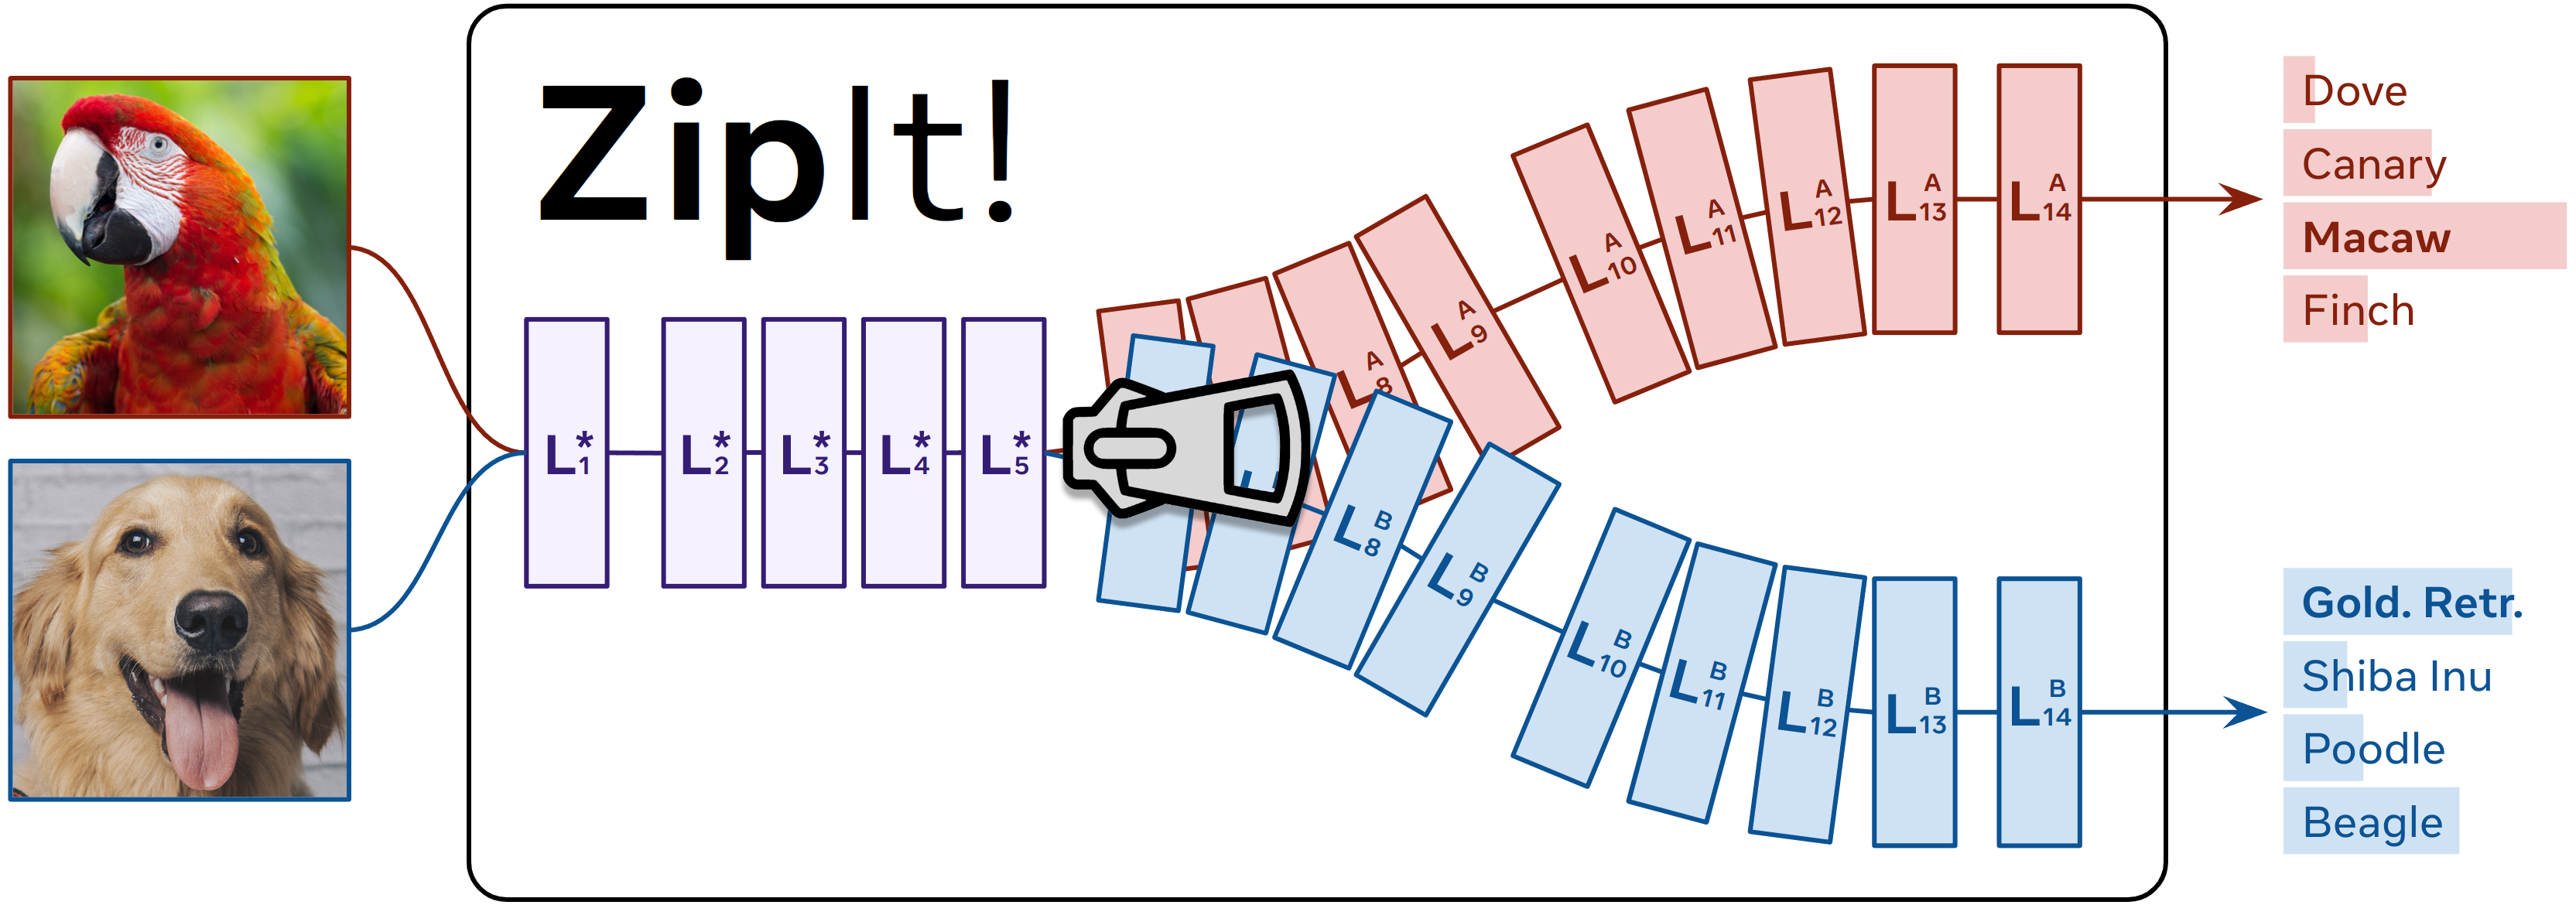
\includegraphics[width=\linewidth]{figures/imgs/concept.png}
%     \caption{{\bf \name{}} merges models trained on completely separate tasks \textit{without any additional training} by identifying their shared features.
%     Depending on the architecture and task, \name{} can nearly match their ensemble performance.
%     }
%     \label{fig:concept}
% }\end{minipage}
% \hspace{1em}
% \begin{minipage}{0.48\linewidth}{
%     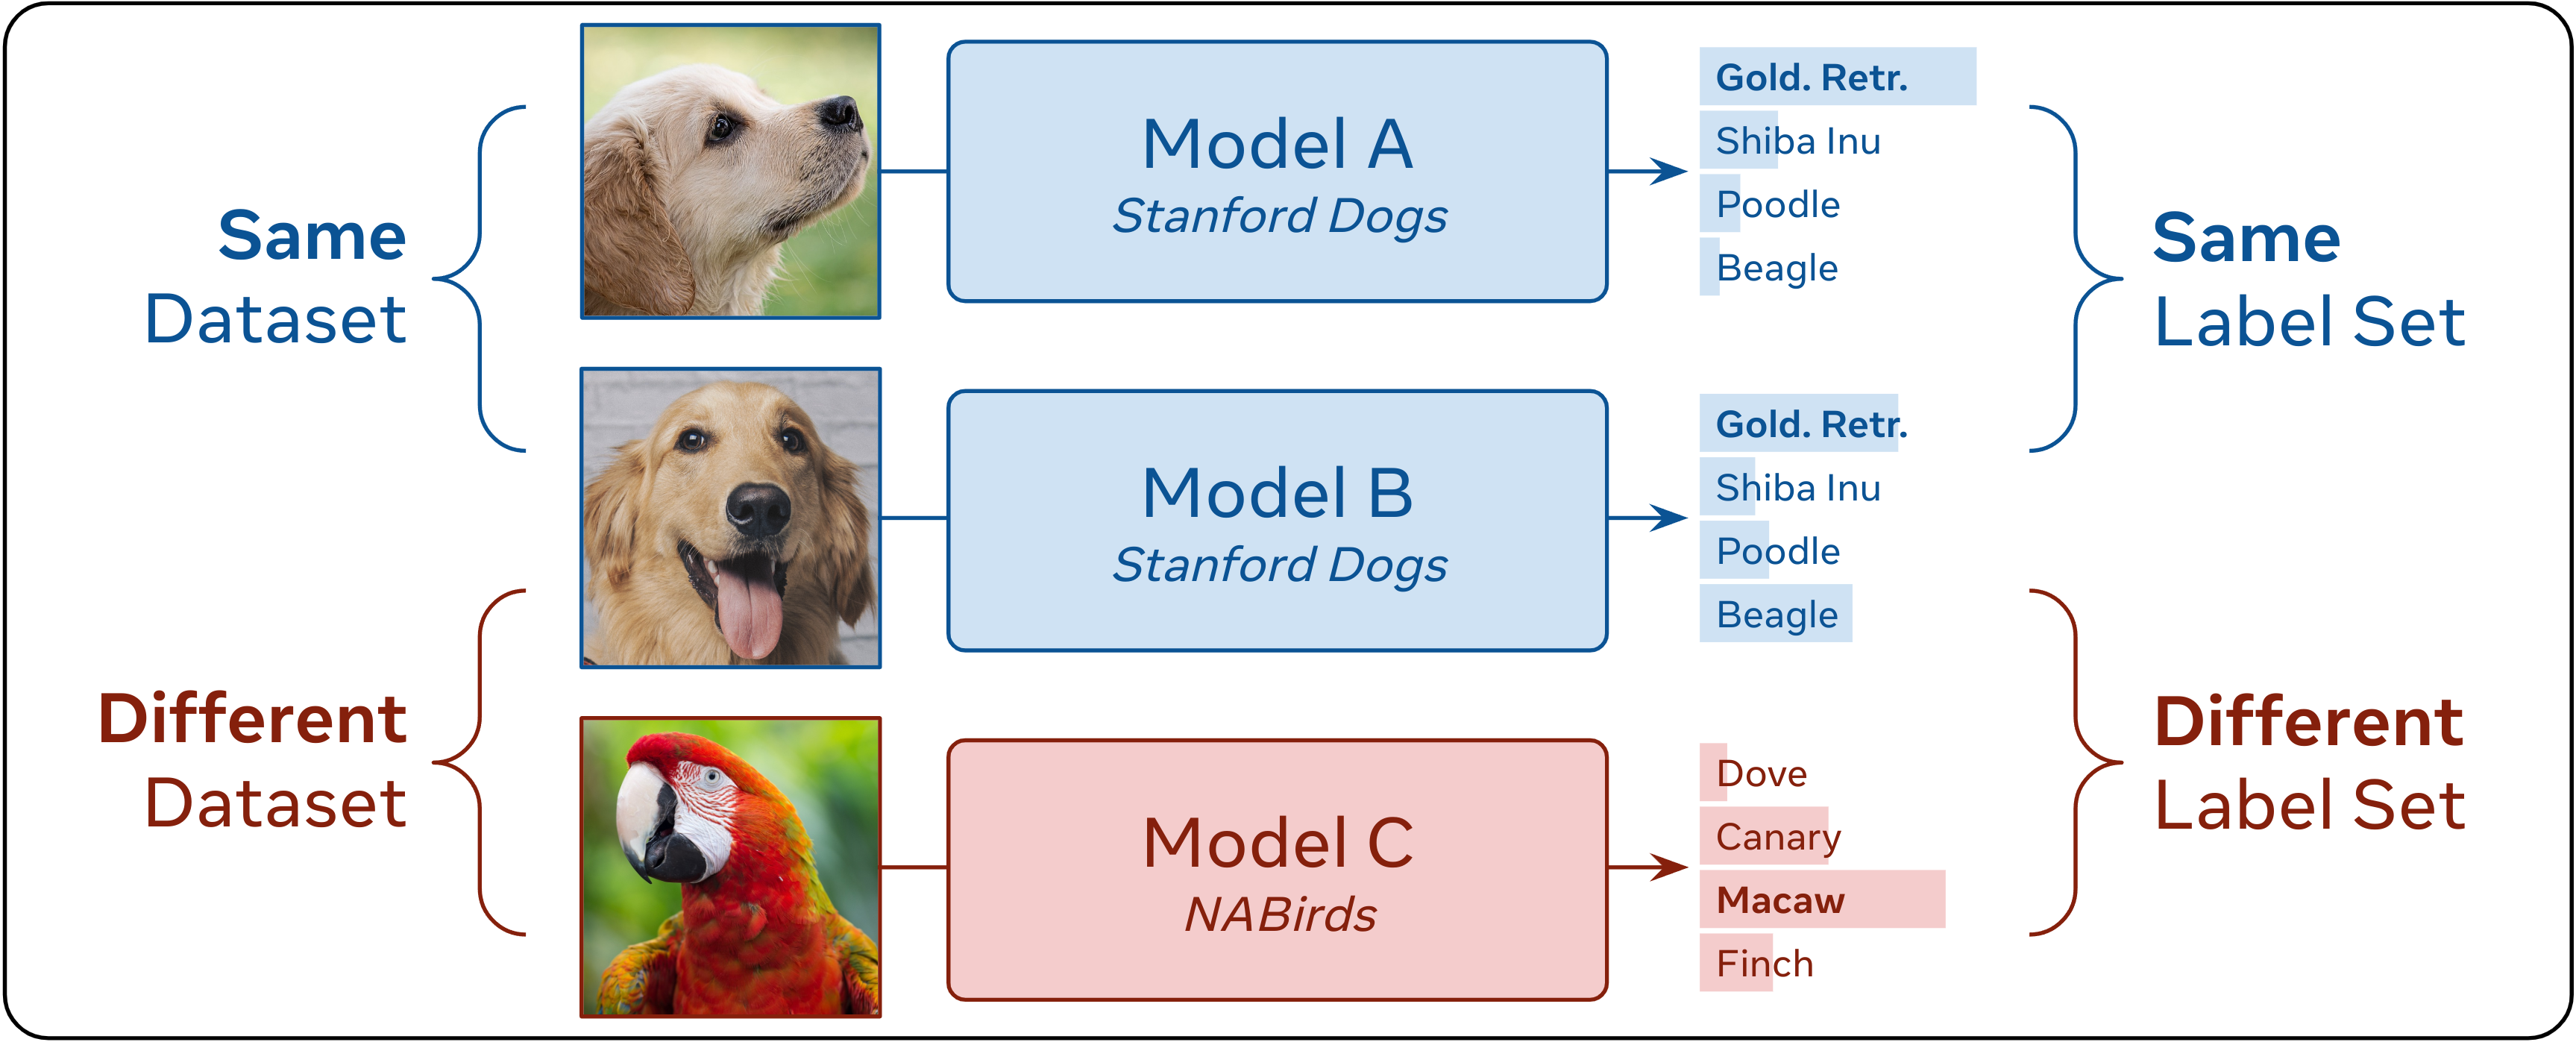
\includegraphics[width=\linewidth]{figures/imgs/vs_prior_work.png}
%     \caption{{\bf Our Setting.} Prior work \cite{wortsman2022model,ainsworth2022git,jordan2022repair}
%     focuses on merging models from the \modelb{\textbf{same} dataset} with the \modelb{\textbf{same} label sets}: e.g., merging two models both trained to classify dog breeds. In this work, we remove that restriction and ``zip'' models that can come from \modela{\textbf{different} datasets} and have \modela{\textbf{different} label sets}: e.g., merging a model that classifies dog breeds with one that classifies bird species.
%     }
%     \label{fig:capabilities}
%     % \includegraphics[width=\linewidth]{figures/imgs/random_r_experiment.png}
    
%     % \captionof{figure}{\textbf{Token Merging Schedule.} Our default constant merging schedule is close to optimal when compared to 15k randomly sampled merging schedules on an AugReg ViT-B/16. }
%     % \label{fig:r_ablation}
% }\end{minipage}
% \end{figure}


% #########################################################

\vspace{-0.5em}
\subsection{CIFAR-10 and CIFAR-100}
We train 5 pairs of ResNet-20 \cite{he2015deep} from scratch with different initializations on disjoint halves of the CIFAR-10 and CIFAR-100 classes \cite{krizhevsky2009cifar}. While \name{}\ supports ``partial zipping'' to merge models with different outputs (in this case, disjoint label sets), prior methods without retraining do not. To make a fair comparison, we train these CIFAR models with a CLIP-style loss \cite{radford2021learning} using CLIP text encodings of the class names as targets. 
This way, both models output into the same CLIP-space regardless of the category.
% That way, both models output into the same space, despite predicting different sets of categories. 
Note, this means the models are capable of some amount of zero-shot classification on the tasks they were not trained on.
% , and can get better than random accuracy on tasks they were not trained on.

% Thus, they get better than random accuracy on tasks they were not trained on.
% We also experiment with VGG models in this setting, and achieve similar results to our ResNet experiments (See Appendix~\ref{ap:vgg}).

\paragraph{CIFAR-10 (5+5).}
In Tab.~\ref{tab:cifar5+5}, we merge models trained on disjoint 5 class subsets of CIFAR-10 using ResNet-20 with a $4\times$ width multiplier (denoted as ResNet-20$\times$4). In joint classification (i.e., 10-way), Git Re-Basin is unable to perform better than using either of the original models alone, while our Permute baseline performs slightly better.
In stark contrast, our \name{}\ performs a staggering \textit{32.9\%} better than Git Re-Basin and \textit{20.7\%} better than our baseline.
If allow the last stage of the network to remain unzipped (i.e., zip up to 13 layers), our method obtains 83.8\%, which is only 3.6\% behind an ensemble of \modela{model A} and \modelb{model B} (which is practically the upper bound for this setting).
We also achieve similar results when merging VGG11 models in this setting (Appendix~\ref{ap:vgg}).

\vspace{-0.2em}
\paragraph{CIFAR-100 (50+50).}
We find similar results on disjoint 50 class splits of CIFAR-100 in Tab.~\ref{tab:cifar50+50}, this time using an $8\times$ width multiplier instead. Like with CIFAR-10, Git Re-Basin fails to outperform even the unmerged models themselves in joint classification (i.e., 100-way), and this time Permute is only 1.2\% ahead. \name{}\ again \textit{significantly} outperforms prior work with +14\% accuracy over Git Re-Basin for all layers zipped, and a substantial +29.2\% if zipping 13/20 layers. At this accuracy, \name{}$_{13/20}$ is again only 3.3\% behind the ensemble for joint accuracy and 2.6\% behind for average per task accuracy, landing itself in an entirely different performance tier compared to prior work.




% %##################################################################################################
\begin{wrapfigure}{r}{0.5\textwidth}
\vspace{-20pt}
\resizebox{0.48\textwidth}{!}{
% \begin{adjustbox}{max width=0.5\textwidth}

    \tablestyle{5pt}{1.1}
    \begin{tabular}{y{53}x{40}|x{30}x{30}x{30}x{30}}
        & & \multicolumn{4}{c}{Accuracies (\%)}\\
        Method & FLOPs (G) & Joint & \modela{Task A} & \modelb{Task B} & Avg \\
        \shline
        \modela{Model A} & {4.11} & {37.2\conf{2.0}} & {74.3\conf{4.0}} & {0.5\conf{0.1}} & {37.4\conf{2.0}} \\
        \modelb{Model B} & {4.11} & {35.3\conf{1.6}} & {0.5\conf{0.1}} & {70.5\conf{3.2}} & {35.5\conf{1.6}} \\
        \hline
        W. Avg \tiny{(Eq.~\ref{eq:wavg})} &4.11& {0.3\conf{0.1}} & {0.6\conf{0.1}} & {0.7\conf{0.1}} & {0.6\conf{0.1}} \\
        Git Re-Basin$^{\ddag}$ &4.11 & {3.1\conf{1.2}} & {5.3\conf{2.6}} & {5.7\conf{2.4}} & {5.5\conf{1.7}}  \\
        % Git Re-Basin \cite{ainsworth2022git}  &4.11 & {3.1\conf{1.2}} & {5.3\conf{2.6}} & {5.7\conf{2.4}} & {5.5\conf{1.7}}  \\
        Permute \tiny{(Eq.~\ref{eq:rebasin})} &4.11 & \textbf{8.6\conf{5.8}} & \textbf{10.1\conf{4.4}} & \textbf{15.3\conf{11.1}} & \textbf{12.7\conf{7.7}} \\
        \default{{\bf \name{}}$_\text{50/50}$} &4.11 & \textbf{8.6\conf{4.7}} & \textbf{12.4\conf{5.9}} & \textbf{14.7\conf{7.8}} & \textbf{13.5\conf{6.6}} \\
        \hline
        \gc{Ensemble} & \gc{8.22} & \gc{63.3\conf{4.9}} & \gc{74.3\conf{4.0}} & \gc{70.5\conf{3.2}} & \gc{72.4\conf{2.5}} \\
        % \default{{\bf \name{}}$_\text{37/50}$} & 4.92 & {33.1\conf{5.9}} & {41.8\conf{5.3}} & {42.3\conf{8.2}} & {42.0\conf{6.2}} \\
        \default{{\bf \name{}}$_\text{22/50}$} & 6.39 & {55.8\conf{4.1}} & {65.9\conf{2.5}} & {64.1\conf{3.0}} & {65.0\conf{2.3}} \\
        \default{{\bf \name{}}$_\text{10/50}$} & 7.43 & \textbf{60.9\conf{4.1}} & \textbf{70.7\conf{3.0}} & \textbf{69.0\conf{2.9}} & \textbf{69.9\conf{1.9}} \\
    \end{tabular}
% \end{adjustbox}
}

\captionof{table}{\textbf{ImageNet-1k (200+200) Results.} Merging ResNet-50 models trained from scratch on disjoint 200 category subsets (Task \modela{A} and \modelb{B}) of ImageNet-1k. Prior work performs poorly, but \name{}\ makes this task feasible. {$^\ddag$\scriptsize \citet{ainsworth2022git}.}
}
\label{tab:imagenet200x5}
\vspace{-14pt}
\end{wrapfigure}
% %##################################################################################################


% %##################################################################################################
% \begin{wrapfigure}{r}{0.5\textwidth}
% % \vspace{-150pt}
% \resizebox{0.48\textwidth}{!}{
% % \begin{adjustbox}{max width=0.5\textwidth}

%     \tablestyle{5pt}{1.1}
%     \begin{tabular}{y{52}x{20}x{28}|x{24}x{24}x{24}}
    
%         & FLOPs& Joint & \multicolumn{3}{c}{Per-Task (\%)}\\
%         Method & (G) & Acc (\%) & \modela{Task A} & \modelb{Task B} & Avg\\
%         \shline
%         \modela{Model A} & {4.11} & {37.2\conf{2.0}} & {74.3\conf{4.0}} & {0.5\conf{0.1}} & {37.4\conf{2.0}} \\
%         \modelb{Model B} & {4.11} & {35.3\conf{1.6}} & {0.5\conf{0.1}} & {70.5\conf{3.2}} & {35.5\conf{1.6}} \\
%         \hline
%         W. Avg \tiny{(Eq.~\ref{eq:wavg})} &4.11& {0.3\conf{0.1}} & {0.6\conf{0.1}} & {0.7\conf{0.1}} & {0.6\conf{0.1}} \\
%         Git Re-Basin$^{\ddag}$ &4.11 & {3.1\conf{1.2}} & {5.3\conf{2.6}} & {5.7\conf{2.4}} & {5.5\conf{1.7}}  \\
%         % Git Re-Basin \cite{ainsworth2022git}  &4.11 & {3.1\conf{1.2}} & {5.3\conf{2.6}} & {5.7\conf{2.4}} & {5.5\conf{1.7}}  \\
%         Permute \tiny{(Eq.~\ref{eq:rebasin})} &4.11 & \textbf{8.6\conf{5.8}} & \textbf{10.1\conf{4.4}} & \textbf{15.3\conf{11.1}} & \textbf{12.7\conf{7.7}} \\
%         \default{{\bf \name{}}$_\text{50/50}$} &4.11 & \textbf{8.6\conf{4.7}} & \textbf{12.4\conf{5.9}} & \textbf{14.7\conf{7.8}} & \textbf{13.5\conf{6.6}} \\
%         \hline
%         \gc{Ensemble} & \gc{8.22} & \gc{63.3\conf{4.9}} & \gc{74.3\conf{4.0}} & \gc{70.5\conf{3.2}} & \gc{72.4\conf{2.5}} \\
%         % \default{{\bf \name{}}$_\text{37/50}$} & 4.92 & {33.1\conf{5.9}} & {41.8\conf{5.3}} & {42.3\conf{8.2}} & {42.0\conf{6.2}} \\
%         \default{{\bf \name{}}$_\text{22/50}$} & 6.39 & {55.8\conf{4.1}} & {65.9\conf{2.5}} & {64.1\conf{3.0}} & {65.0\conf{2.3}} \\
%         \default{{\bf \name{}}$_\text{10/50}$} & 7.43 & \textbf{60.9\conf{4.1}} & \textbf{70.7\conf{3.0}} & \textbf{69.0\conf{2.9}} & \textbf{69.9\conf{1.9}} \\
%     \end{tabular}
% % \end{adjustbox}
% }

% \caption{\textbf{ImageNet-1k (200+200) Results.} Merging ResNet-50 models trained from scratch on disjoint 200 category subsets (Task \modela{A} and \modelb{B}) of ImageNet-1k. Prior work performs poorly, but \name{}\ makes this task feasible. $\ddag$ refers to \cite{ainsworth2022git}
% }
% \label{tab:imagenet200x5}
% \end{wrapfigure}
% %##################################################################################################
\vspace{-0.5em}
\subsection{ImageNet-1k (200+200)}
To test our method on the \textit{much harder} setting of large-scale data, we train 5 differently initialized ResNet-50 models with cross entropy loss on disjoint 200 class subsets of ImageNet-1k \cite{deng2009imagenet}.
To compare to prior work that doesn't support partial zipping, we initialize the models with capacity for all 1k classes, but only train each on their subset.

In Tab.~\ref{tab:imagenet200x5} we show results on exhaustively merging pairs from the 5 models. To compute joint (i.e., 400-way) accuracy, we softmax over each task's classes individually (like in \citet{ahn2021ss}), and take the argmax over the combined 400 class vector. On this extremely difficult task, Git Re-Basin only obtains 3.1\% for joint accuracy (with random accuracy being 0.25\%).
Both the Permute baseline and \name{}\ with all layers zipped perform better, but with each at 8.6\%, are still clearly lacking.
Note that we find the same-model merging budget $\beta$ to not matter for this set of models (see Fig.~\ref{fig:variations}), which suggests that there's not a lot of redundant information \textit{within} each model 
% for
in
this setting. Thus, \name{}\ chooses to merge mostly \textit{across} models instead, performing similarly to the permute baseline. We find this same trend in CIFAR with smaller models (see Fig.~\ref{fig:variations}), 
% so this 
and
may be an artifact of model capacity. 
% To that end, 
The story changes when we increase the capacity of the merged model by partial zipping: \name{}$_{10/50}$ 
% is able to reach 
reaches
close to upper bound ensemble accuracy \textit{on this extremely difficult task}, while saving on FLOPs.

\vspace{-0.5em}
\subsection{Multi-Dataset Merging}
We now take our model merging framework one step further by merging differently initialized models trained on \textit{completely separate datasets and tasks}. We present two settings: merging multiple classification datasets and merging semantic segmentation with image classification.

% in one we merge image classification models, and in the other we merge image generation models.
% We first present a setting where we merge models trained on different image classification datasets, and second a setting where we merge several image generation models.

% % Concatenated Table
% %##################################################################################################
% \begin{table*}[t]
% \centering
% \subfloat[
%     \textbf{Merging Model Pairs.} ResNet-50.
%     \label{tab:two_way}
% ]{
% \centering
% \begin{minipage}{0.47\linewidth}{
% \begin{center}
% \resizebox{\textwidth}{!}{
%     \tablestyle{5pt}{1.1}
%     {\renewcommand\conf[1]{}
%     \tablestyle{5pt}{1.1}
%     \begin{tabular}{y{50}x{40}|x{20}x{20}x{20}x{20}x{20}}
%         & & \multicolumn{5}{c}{Paired-Merge Per-Task Accuracies (\%)} \\
%         Method & FLOPs (G) & SD & OP & CUB & NAB & Avg\\
%         \shline
%         W. Avg \tiny{(Eq.~\ref{eq:wavg})} & {4.11} & {15.1\conf{18.8}} & {23.8\conf{43.3}} & {11.8\conf{19.2}} & {2.1\conf{3.2}} & {13.2\conf{9.0}}  \\
%         Permute \tiny{(Eq.~\ref{eq:rebasin})} & 4.11 & \textbf{51.3\conf{10.6}} & 64.7\conf{15.3} & 36.7\conf{17.8} & \textbf{15.5\conf{64.7}} & 42.1\conf{21.1} \\
%         \default{{\bf \name{}}$_\text{49/50}$} & 4.11 & \textbf{51.2\conf{9.4}} & \textbf{67.7\conf{17.6}} & \textbf{40.6\conf{19.1}} & \textbf{15.6\conf{12.2}} & \textbf{43.8\conf{21.8}} \\
%         \hline
%         \gc{Ensemble} & \gc{8.22} & \gc{72.7} & \gc{83.2} & \gc{71.0} & \gc{77.2} & \gc{76.0\conf{4.7}} \\
%         \default{{\bf \name{}}$_\text{37/50}$} & 4.92 & {56.8\conf{1.9}} & {73.8\conf{13.1}} & {54.6\conf{3.5}} & {37.9\conf{22.3}} & {55.8\conf{14.7}} \\
%         \default{{\bf \name{}}$_\text{22/50}$} & 6.39 & \textbf{65.3\conf{0.6}} & \textbf{79.7\conf{4.8}} & \textbf{64.8\conf{2.2}} & \textbf{61.2\conf{8.9}} & \textbf{67.7\conf{8.2}} \\
%     \end{tabular}
%     }
% }
% \end{center}
% }\end{minipage}
% }
% \hspace{1em}
% \centering
% \subfloat[
%     \textbf{Merging All Models.} ResNet-50.
%     \label{tab:cifar50+50}
% ]{
% \centering
% \begin{minipage}{0.47\linewidth}{
% \begin{center}
% \resizebox{\textwidth}{!}{
%     \tablestyle{5pt}{1.1}
%     {\renewcommand\conf[1]{}
%     \tablestyle{5pt}{1.1}
%     \begin{tabular}{y{50}x{40}|x{20}x{20}x{20}x{20}x{20}}
%         & & \multicolumn{5}{c}{All-Merged Per-Task Accuracies (\%)} \\
%         Method & FLOPs (G) & SD & OP & CUB & NAB & Avg\\
%         \shline
%         W. Avg \tiny{(Eq.~\ref{eq:wavg})} & {4.12} & {0.7} & {3.4} & {0.4} & {0.2} & {1.2\conf{1.5}}  \\
%         Permute \tiny{(Eq.~\ref{eq:rebasin})} & {4.12} & \textbf{34.2} & \textbf{55.4} & {13.4} & {5.7} & \textbf{27.2\conf{19.3}}  \\
%         \default{{\bf \name{}}$_\text{49/50}$} & {4.12} & {32.1} & \textbf{55.3} & \textbf{14.7} & \textbf{6.9} & \textbf{27.3\conf{20.1}}  \\
%         \hline
%         \gc{Ensemble} & \gc{16.44} & \gc{72.7} & \gc{83.2} & \gc{71.0} & \gc{77.2} & \gc{76.0\conf{4.7}} \\
%         \default{{\bf \name{}}$_\text{37/50}$} & {6.5} & {39.9} & {66.4} & {44.3} & {24.6} & {43.8\conf{17.2}}  \\
%         \default{{\bf \name{}}$_\text{22/50}$} & {11.0} & \textbf{58.2} & \textbf{78.5} & \textbf{58.6} & \textbf{55.1} & \textbf{62.6\conf{10.7}}  \\
%     \end{tabular}
%     }
% }
% \end{center}
% }\end{minipage}
% }
% \caption{\textbf{Multi-Dataset Results.} Merge differently initialized ResNet-50 models trained on \textit{disjoint datasets}: Stanford Dogs (SD), Oxford Pets (OP), CUB200 (CUB), and NABirds (NAB). 
% % We report average per-task accuracy over merging model pairs, and merging all four.
% }
% \label{tab:cross_dataset_results}
% % \vspace{-15pt}
% \end{table*}
%##################################################################################################
% Imnet200 P1 Table
% Stacked Table
%##################################################################################################

\begin{wrapfigure}{r}{0.48\linewidth}
\vspace{-20pt}
\centering
\resizebox{\linewidth}{!}{
    \tablestyle{5pt}{1.1}
    {\renewcommand\conf[1]{}
    \tablestyle{5pt}{1.1}
    \begin{tabular}{y{50}x{40}|x{20}x{20}x{20}x{20}x{20}}
        & & \multicolumn{5}{c}{Per-Task Accuracies (\%)} \\
        Method & FLOPs (G) & SD & OP & CUB & NAB & Avg\\
        \shline
        \multicolumn{7}{c}{Merging Pairs}\\
        \hline                                % FLOPS       Stanford Dogs               Oxford Pets                 CUB                         NA Birds                    Avg
        W. Avg \tiny{(Eq.~\ref{eq:wavg})}       & 4.11      & {12.9\conf{18.8}}         & {18.2\conf{43.3}}         & {13.9\conf{19.2}}         & {0.2\conf{3.2}}           & {11.3\conf{0.0}}  \\
        Permute \tiny{(Eq.~\ref{eq:rebasin})}   & 4.11      & 46.2\conf{15.5}            & 47.6\conf{16.6}           & 35.6\conf{24.7}           & \textbf{13.5\conf{14.9}}  & 35.7\conf{0.} \\
        \default{{\bf \name{}}$_\text{49/50}$}  & 4.11      & \textbf{46.9\conf{7.2}}   & \textbf{50.7\conf{13.0}}  & \textbf{38.0\conf{21.5}} & 12.7\conf{14.6}           & \textbf{37.1\conf{0}} \\
        \hline
        \gc{Ensemble}                           & \gc{8.22} & \gc{72.7}                 & \gc{81.1}                 & \gc{71.0}                 & \gc{77.2}                 & \gc{75.5\conf{4.7}} \\
        % \default{{\bf \name{}}$_\text{37/50}$}  & 4.92      & {53.9\conf{3.8}}          & {59.6\conf{6.0}}          & {52.8\conf{9.3}}         & {21.1\conf{14.4}}         & {46.9\conf{0.}} \\
        \default{{\bf \name{}}$_\text{22/50}$}  & 6.39      & {62.6\conf{2.3}}          & {71.2\conf{2.1}}          & {62.8\conf{5.3}}          & {53.0\conf{8.4}}          & {62.4\conf{0.}} \\
        \default{{\bf \name{}}$_\text{10/50}$}  & 7.42      & \textbf{66.5\conf{1.5}}   & \textbf{75.8\conf{1.9}}   & \textbf{65.6\conf{3.7}}   & \textbf{66.8\conf{4.0}}   & \textbf{68.7\conf{0.}} \\
        \hline
        \multicolumn{7}{c}{Merging All 4}\\
        \hline
        W. Avg \tiny{(Eq.~\ref{eq:wavg})}       & {4.12}    & {0.8}                     & {3.0}                     & {0.6}                     & {0.3}                     & {1.2\conf{1.5}}  \\
        Permute \tiny{(Eq.~\ref{eq:rebasin})}   & {4.12}    & {15.7}                    & {26.1}                    & \textbf{14.0}             & \textbf{5.3}              & {15.3\conf{19.3}}  \\
        \default{{\bf \name{}}$_\text{49/50}$}  & {4.12}    & \textbf{21.1}             & \textbf{33.3}             & {8.6}                     & {3.9}                     & \textbf{16.8\conf{20.1}}  \\
        \hline
        \gc{Ensemble}                           & \gc{16.4}& \gc{72.7}                 & \gc{81.2}                 & \gc{71.0}                 & \gc{77.2}                 & \gc{75.5\conf{4.7}} \\
        % \default{{\bf \name{}}$_\text{37/50}$}  & {6.5}     & {29.2}                    & {38.6}                    & {24.7}                    & {10.5}                    & {25.8\conf{17.2}}  \\
        \default{{\bf \name{}}$_\text{22/50}$}  & {11.0}    & {50.2}                    & {55.9}                    & {44.0}                    & {32.0}                    & {45.5\conf{10.7}}  \\
        \default{{\bf \name{}}$_\text{10/50}$}  & {14.1}    & \textbf{63.5}             & \textbf{70.8}             & \textbf{63.7}             & \textbf{63.1}             & \textbf{65.3\conf{10.7}}  \\
    \end{tabular}
    }
}
\captionof{table}{\textbf{Multi-Dataset Results.} Merging 
% differently initialized 
ResNet-50 models trained on \textit{completely different datasets}: Stanford Dogs (SD), Oxford Pets (OP), CUB200 (CUB), and NABirds (NAB). We report average per-task accuracy over merging model pairs, and all four.
% all pairs (2-way merging) and per-task accuracy for each head (4-way merging).
% We compare to our strong baseline as \cite{ainsworth2022git} doesn't support models with different outputs.
}
\label{tab:cross_dataset_results}
% \end{table}
\vspace{-20pt}
\end{wrapfigure}
% ##################################################################################################

% Table Partially filled in with Innet200 P0
% % Stacked Table
% %##################################################################################################

% \begin{wrapfigure}{r}{0.48\linewidth}
% \vspace{-10pt}
% \centering
% \resizebox{\linewidth}{!}{
%     \tablestyle{5pt}{1.1}
%     {\renewcommand\conf[1]{}
%     \tablestyle{5pt}{1.1}
%     \begin{tabular}{y{50}x{40}|x{20}x{20}x{20}x{20}x{20}}
%         & & \multicolumn{5}{c}{Per-Task Accuracies (\%)} \\
%         Method & FLOPs (G) & SD & OP & CUB & NAB & Avg\\
%         \shline
%         \multicolumn{7}{c}{Merging Pairs}\\
%         \hline
%         W. Avg \tiny{(Eq.~\ref{eq:wavg})} & {4.11} & {12.9\conf{18.8}} & {18.2\conf{43.3}} & {13.9\conf{19.2}} & {0.2\conf{3.2}} & {11.3\conf{9.0}}  \\
%         Permute \tiny{(Eq.~\ref{eq:rebasin})} & 4.11 & 46.2\conf{15.5} & 47.6\conf{16.6} & 35.6\conf{24.7} & \textbf{13.5\conf{14.9}} & 35.7\conf{21.1} \\
%         \default{{\bf \name{}}$_\text{49/50}$} & 4.11 & \textbf{46.9\conf{7.2}} & \textbf{50.7\conf{13.0}} & \textbf{38.0\conf{21.5}} & 12.7\conf{14.6} & \textbf{37.1\conf{21.8}} \\
%         \hline
%         \gc{Ensemble} & \gc{8.22} & \gc{72.7} & \gc{81.1} & \gc{71.0} & \gc{77.2} & \gc{76.0\conf{4.7}} \\
%         \default{{\bf \name{}}$_\text{37/50}$} & 4.92 & {53.9\conf{1.9}} & {59.6\conf{13.1}} & {52.8\conf{3.5}} & {21.1\conf{22.3}} & {46.9\conf{14.7}} \\
%         \default{{\bf \name{}}$_\text{22/50}$} & 6.39 & \textbf{62.6\conf{0.6}} & \textbf{71.2\conf{4.8}} & \textbf{62.8\conf{2.2}} & \textbf{53.0\conf{8.9}} & \textbf{62.4\conf{8.2}} \\
%         \hline
%         \multicolumn{7}{c}{Merging All 4}\\
%         \hline
%         W. Avg \tiny{(Eq.~\ref{eq:wavg})} & {4.12} & {0.7} & {3.4} & {0.4} & {0.2} & {1.2\conf{1.5}}  \\
%         Permute \tiny{(Eq.~\ref{eq:rebasin})} & {4.12} & \textbf{15.7} & \textbf{26.1} & {14.0} & {5.3} & \textbf{15.3\conf{19.3}}  \\
%         \default{{\bf \name{}}$_\text{49/50}$} & {4.12} & {32.1} & \textbf{55.3} & \textbf{14.7} & \textbf{6.9} & \textbf{27.3\conf{20.1}}  \\
%         \hline
%         \gc{Ensemble} & \gc{16.44} & \gc{72.7} & \gc{83.2} & \gc{71.0} & \gc{77.2} & \gc{76.0\conf{4.7}} \\
%         \default{{\bf \name{}}$_\text{37/50}$} & {6.5} & {39.9} & {66.4} & {44.3} & {24.6} & {43.8\conf{17.2}}  \\
%         \default{{\bf \name{}}$_\text{22/50}$} & {11.0} & \textbf{58.2} & \textbf{78.5} & \textbf{58.6} & \textbf{55.1} & \textbf{62.6\conf{10.7}}  \\
%     \end{tabular}
%     }
% }
% \captionof{table}{\textbf{Multi-Dataset Results.} Merging 
% % differently initialized 
% ResNet-50 models trained on \textit{completely different datasets}: Stanford Dogs (SD), Oxford Pets (OP), CUB200 (CUB), and NABirds (NAB). We report average per-task accuracy over merging model pairs, and all four.
% % all pairs (2-way merging) and per-task accuracy for each head (4-way merging).
% % We compare to our strong baseline as \cite{ainsworth2022git} doesn't support models with different outputs.
% }
% \label{tab:cross_dataset_results}
% % \end{table}
% \vspace{-20pt}
% \end{wrapfigure}
% % ##################################################################################################





% \begin{wrapfigure}{r}{0.48\linewidth}
% \vspace{-260pt}
% % \begin{minipage}{0.48\linewidth}{
% %     \centering
% %     \resizebox{\textwidth}{!}{
% %         \tablestyle{5pt}{1.1}
% %         {\renewcommand\conf[1]{}
% %         \tablestyle{5pt}{1.1}
% %         \begin{tabular}{y{50}x{20}|x{20}x{20}x{20}x{20}x{20}}
% %             & FLOPs & \multicolumn{5}{c}{Per-Task (\%)} \\
% %             Method & (G) & SD & OP & CUB & NAB & Avg\\
% %             \shline
% %             \multicolumn{7}{c}{Merging Pairs}\\
% %             \hline
% %             W. Avg \tiny{(Eq.~\ref{eq:wavg})} & {4.11} & {15.1\conf{18.8}} & {23.8\conf{43.3}} & {11.8\conf{19.2}} & {2.1\conf{3.2}} & {13.2\conf{9.0}}  \\
% %             Permute \tiny{(Eq.~\ref{eq:rebasin})} & 4.11 & \textbf{51.3\conf{10.6}} & 64.7\conf{15.3} & 36.7\conf{17.8} & \textbf{15.5\conf{64.7}} & 42.1\conf{21.1} \\
% %             \default{{\bf \name{}}$_\text{49/50}$} & 4.11 & \textbf{51.2\conf{9.4}} & \textbf{67.7\conf{17.6}} & \textbf{40.6\conf{19.1}} & \textbf{15.6\conf{12.2}} & \textbf{43.8\conf{21.8}} \\
% %             \hline
% %             \gc{Ensemble} & \gc{8.22} & \gc{72.7} & \gc{83.2} & \gc{71.0} & \gc{77.2} & \gc{76.0\conf{4.7}} \\
% %             \default{{\bf \name{}}$_\text{37/50}$} & 4.92 & {56.8\conf{1.9}} & {73.8\conf{13.1}} & {54.6\conf{3.5}} & {37.9\conf{22.3}} & {55.8\conf{14.7}} \\
% %             \default{{\bf \name{}}$_\text{22/50}$} & 6.39 & \textbf{65.3\conf{0.6}} & \textbf{79.7\conf{4.8}} & \textbf{64.8\conf{2.2}} & \textbf{61.2\conf{8.9}} & \textbf{67.7\conf{8.2}} \\
% %             \hline
% %             \multicolumn{7}{c}{Merging All 4}\\
% %             \hline
% %             W. Avg \tiny{(Eq.~\ref{eq:wavg})} & {4.12} & {0.7} & {3.4} & {0.4} & {0.2} & {1.2\conf{1.5}}  \\
% %             Permute \tiny{(Eq.~\ref{eq:rebasin})} & {4.12} & \textbf{34.2} & \textbf{55.4} & {13.4} & {5.7} & \textbf{27.2\conf{19.3}}  \\
% %             \default{{\bf \name{}}$_\text{49/50}$} & {4.12} & {32.1} & \textbf{55.3} & \textbf{14.7} & \textbf{6.9} & \textbf{27.3\conf{20.1}}  \\
% %             \hline
% %             \gc{Ensemble} & \gc{16.44} & \gc{72.7} & \gc{83.2} & \gc{71.0} & \gc{77.2} & \gc{76.0\conf{4.7}} \\
% %             \default{{\bf \name{}}$_\text{37/50}$} & {6.5} & {39.9} & {66.4} & {44.3} & {24.6} & {43.8\conf{17.2}}  \\
% %             \default{{\bf \name{}}$_\text{22/50}$} & {11.0} & \textbf{58.2} & \textbf{78.5} & \textbf{58.6} & \textbf{55.1} & \textbf{62.6\conf{10.7}}  \\
% %         \end{tabular}
% %         }
% %     }
% %     \captionof{table}{\textbf{Multi-Dataset Results.} Merging pairs of differently initialized ResNet-50 models trained on \textit{completely different datasets}: Stanford Dogs (SD), Oxford Pets (OP), CUB200 (CUB), and NABirds (NAB). We report average per-task accuracy over all pairs (2-way merging) and per-task accuracy for each head (4-way merging).
% %     We compare to our strong baseline as \cite{ainsworth2022git} doesn't support models with different outputs.
% %     }
% %     \label{tab:cross_dataset_results}
% %     % \end{table}

% % }\end{minipage}
% % \hfill

% \begin{minipage}[c]{\linewidth}{

%     \begin{minipage}[c]{\linewidth}
%         \resizebox{\textwidth}{!}{
%         % \begin{adjustbox}{max width=0.5\textwidth}
        
%             \tablestyle{5pt}{1.1}
%             \begin{tabular}{y{53}x{40}|x{30}x{30}x{30}x{30}}
%                 & & \multicolumn{4}{c}{Accuracies (\%)}\\
%                 Method & FLOPs (G) & Joint & \modela{Task A} & \modelb{Task B} & Avg \\
%                 \shline
%                 \modela{Model A} & {4.11} & {37.2\conf{2.0}} & {74.3\conf{4.0}} & {0.5\conf{0.1}} & {37.4\conf{2.0}} \\
%                 \modelb{Model B} & {4.11} & {35.3\conf{1.6}} & {0.5\conf{0.1}} & {70.5\conf{3.2}} & {35.5\conf{1.6}} \\
%                 \hline
%                 W. Avg \tiny{(Eq.~\ref{eq:wavg})} &4.11& {0.3\conf{0.1}} & {0.6\conf{0.1}} & {0.7\conf{0.1}} & {0.6\conf{0.1}} \\
%                 Git Re-Basin$^{\ddag}$ &4.11 & {3.1\conf{1.2}} & {5.3\conf{2.6}} & {5.7\conf{2.4}} & {5.5\conf{1.7}}  \\
%                 % Git Re-Basin \cite{ainsworth2022git}  &4.11 & {3.1\conf{1.2}} & {5.3\conf{2.6}} & {5.7\conf{2.4}} & {5.5\conf{1.7}}  \\
%                 Permute \tiny{(Eq.~\ref{eq:rebasin})} &4.11 & \textbf{8.6\conf{5.8}} & \textbf{10.1\conf{4.4}} & \textbf{15.3\conf{11.1}} & \textbf{12.7\conf{7.7}} \\
%                 \default{{\bf \name{}}$_\text{50/50}$} &4.11 & \textbf{8.6\conf{4.7}} & \textbf{12.4\conf{5.9}} & \textbf{14.7\conf{7.8}} & \textbf{13.5\conf{6.6}} \\
%                 \hline
%                 \gc{Ensemble} & \gc{8.22} & \gc{63.3\conf{4.9}} & \gc{74.3\conf{4.0}} & \gc{70.5\conf{3.2}} & \gc{72.4\conf{2.5}} \\
%                 % \default{{\bf \name{}}$_\text{37/50}$} & 4.92 & {33.1\conf{5.9}} & {41.8\conf{5.3}} & {42.3\conf{8.2}} & {42.0\conf{6.2}} \\
%                 \default{{\bf \name{}}$_\text{22/50}$} & 6.39 & {55.8\conf{4.1}} & {65.9\conf{2.5}} & {64.1\conf{3.0}} & {65.0\conf{2.3}} \\
%                 \default{{\bf \name{}}$_\text{10/50}$} & 7.43 & \textbf{60.9\conf{4.1}} & \textbf{70.7\conf{3.0}} & \textbf{69.0\conf{2.9}} & \textbf{69.9\conf{1.9}} \\
%             \end{tabular}
%         % \end{adjustbox}
%         }
        
%         \caption{\textbf{ImageNet-1k (200+200) Results.} Merging ResNet-50 models trained from scratch on disjoint 200 category subsets (Task \modela{A} and \modelb{B}) of ImageNet-1k. Prior work performs poorly, but \name{}\ makes this task feasible. $\ddag$ refers to \cite{ainsworth2022git}
%         }
%         \label{tab:imagenet200x5}
%     \end{minipage}
%     \begin{minipage}[c]{\linewidth}
%         \centering
%         \resizebox{\textwidth}{!}{
%             \tablestyle{7pt}{1.05}
%             \begin{tabular}{y{55}x{43}x{22}x{30}}
%                 Algorithm & \modela{A}$\leftrightarrow$\modela{A}/\modelb{B}$\leftrightarrow$\modelb{B}? & Acc & Time\\
%                 \shline
%                 Identity {\scriptsize (Eq.~\ref{eq:wavg})}                  & \xmark{} & {43.0\conf{3.1}} & {1.8\unit{ms}} \\
%                 Permute {\scriptsize (Eq.~\ref{eq:rebasin})}                & \xmark{} & {58.4\conf{1.3}} & {28\unit{ms}} \\
%                 K-Means                                                     & \checkmark{} & {29.1\conf{5.5}} & {19\unit{sec}} \\
%                 \hline
%                 \multicolumn{4}{c}{Zip {\scriptsize (Eq.~\ref{eq:zip})}} \\
%                 Optimal Match                                               & \checkmark{} & {\bf 79.6\conf{1.7}} & {11\unit{min}} \\
%                 Greedy Match                                                & \checkmark{} & {\bf 79.0\conf{1.8}} & {1.1\unit{sec}} \\
%                 Greedy, $\alpha$=0.1 & \default{\checkmark{}} & \default{\textbf{79.1\conf{2.1}}}  &  \default{1.2\unit{sec}}  \\
%             \end{tabular}
%         }
%         \captionof{table}{{\bf Matching Algorithm} to use for \modelc{$M_i$}. 
%         Permuting \modelb{B}$\rightarrow$\modela{A} as in prior work (Eq.~\ref{eq:rebasin}) performs poorly, thus we allow merging features \textit{within} each model (Eq.~\ref{eq:zip}).
%         Our greedy approach is nearly as accurate as the optimal algorithm while being two orders of magnitude faster. 
%         ``Acc'' is CIFAR-10 (5+5) joint 10-way accuracy.
%         }
%         \label{tab:matching_alg}
%     \end{minipage}
%     \vspace{10pt}
%     \begin{minipage}[c]{\linewidth}
%         % \vspace{40pt}
%         \centering
%         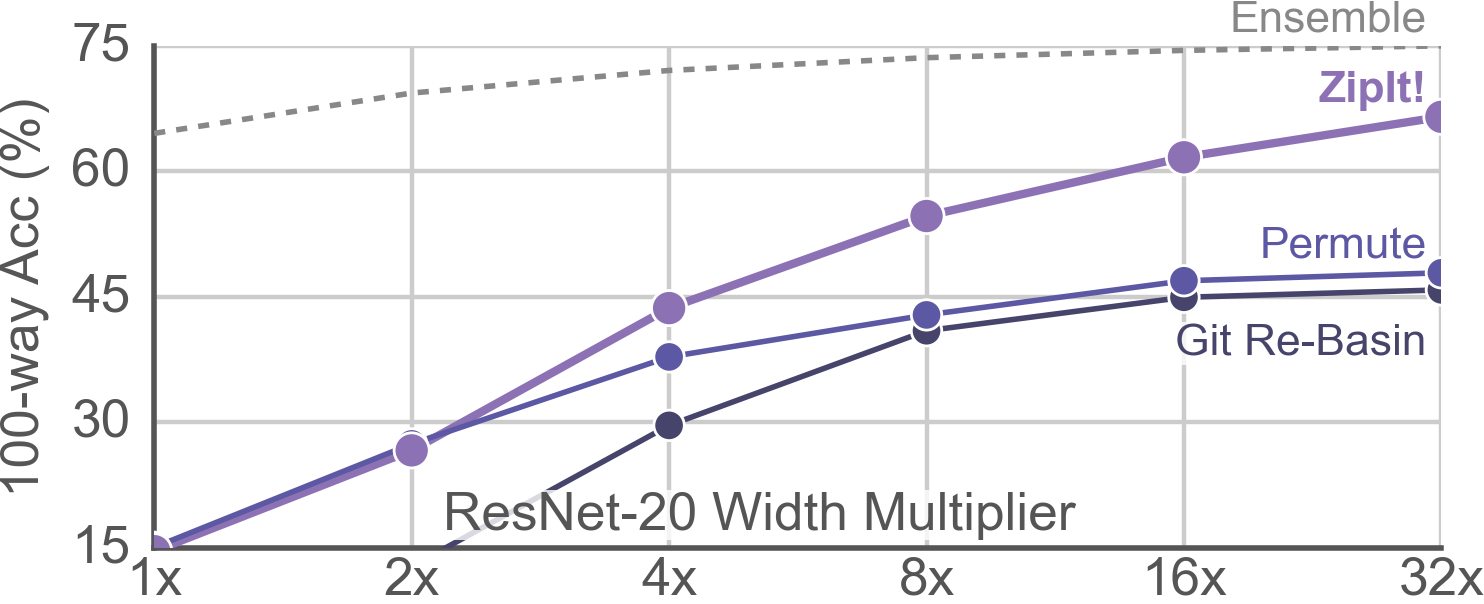
\includegraphics[width=0.95\linewidth]{figures/imgs/model_scale.png}
%         \caption{{\bf Model Scale.} As we increase the width of the ResNet-20 models used for the CIFAR-100 (50+50) setting, \name{}\ makes effective use of that extra capacity, quickly approaching ensemble accuracy. 
%         Git Re-Basin \cite{ainsworth2022git} and Permute only slightly benefit from the extra scale.
%         }
%         \label{fig:model_size}
%         % \vspace{-60pt}
%     \end{minipage}
% }\end{minipage}
% \end{wrapfigure}

\paragraph{Image Classification Datasets.}
% In this experiment, we take disjoint task model merging one step further by merging ResNet-50 models with different initializations trained on \textbf{four} \textit{completely separate datasets}, each with a different set of labels
Merging ResNet-50 models trained on: Stanford Dogs \cite{khosla2011stanforddogs}, Oxford Pets \cite{parkhi2012oxfordpets}, CUB200 \cite{welinder2010cub200}, and NABirds \cite{van2015buildingNaBird}. In Tab.~\ref{tab:cross_dataset_results},
we show the average per task accuracy from exhaustively merging each pair and the much more difficult setting of merging all four at once.
% we show the average per task accuracy for each dataset both if we exhaustively merge each pair and also the much more difficult setting of merging all four at once. 
We report the accuracy of our baselines by applying them up until the last layer, but we can't compare to prior work as they don't support this setting. As in all our previous experiment we merge \textit{without retraining}.

For pairs of models, \name{}\ slightly outperforms our permute baseline across all tasks and performs similarly when merging all 4 models at once.
% And for merging all 4 models at once, we perform similarly to permuting. 
However, if we add capacity to the merged model through partial zipping, we perform up to 33\% better on merging pairs and 50\% better on merging all four models than the permute baseline. Partial zipping is a significant factor to obtain strong performance, especially with more than 2 models.

\paragraph{Multiple Output Modalities.} In Appendix~\ref{appendix:semantic_segmentation}, we combine across modalities by merging the ResNet-50 backbone of a DeeplabV3 \cite{chen2017deeplabv3} segmentation model with an ImageNet-1k classification model. The resulting combined model can perform both semantic segmentation and image classification. Even with half of layers merged, \name{}\ retains good performance on both tasks.
